\chapter{Introduction} \label{Nuclear_DVCS}
\section{DVCS off Helium-4} \label{Nuclear_DVCS}
Nuclear targets provide access to the measurement of two DVCS channels: the coherent and the incoherent. In the coherent channel, the target nucleus remains intact and recoils as a whole while emitting a real photon ($eA \rightarrow e' A' \gamma$). This process allows to measure the nuclear GPDs of the target, which contain information on the partons correlations and the nuclear forces in the target \cite{M_Polyakov,EMC_simonetta}. In the incoherent channel, the nucleus breaks up and the DVCS takes place on a bound nucleon that emits the final photon ($eA \rightarrow e' N' \gamma$ X). The latter allows to measure the GPDs of the bound nucleons and study the medium modifications of the nucleons in the nuclear medium. Figure \ref{fig:nuclear_DVCS} shows the diagrams of the two DVCS channels. 
\begin{figure}[tbp]
\centering
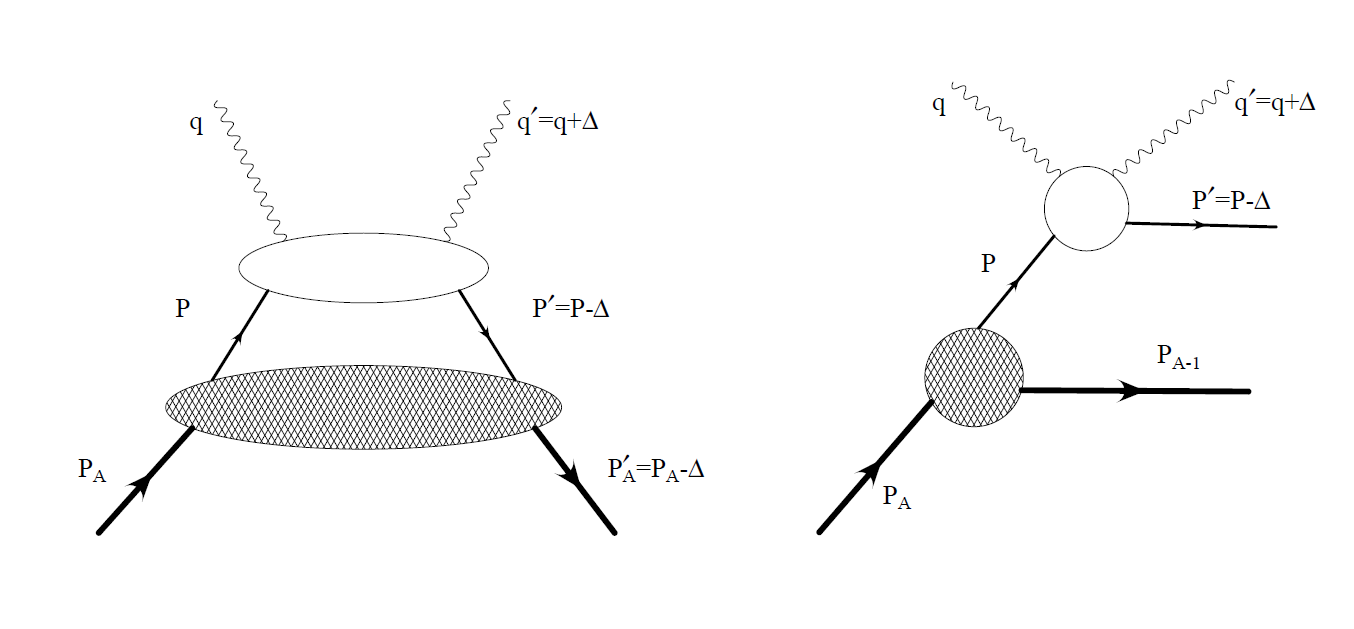
\includegraphics[scale=0.3]{fig/nuclear_DVCS.png}
\caption{The leading twist handbag diagrams of the two DVCS channels from a nuclear target, coherent channel (on the left) and incoherent channel (on the right). } 
\label{fig:nuclear_DVCS}
\end{figure}

The GPDs depend on three variables: $x$, $\xi$ and $t$. $x+\xi$ is the 
nucleon's longitudinal momentum fraction carried by the struck quark, 2$\xi$ is 
the longitudinal momentum fraction of the momentum transfer $\Delta$ ($= p' - 
p$), and $t$ (=$\Delta^{2}$) is the squared momentum transfer between the 
initial and the final states of the hadron target. Experimentally, only $\xi$ 
and $t$ are measurable in the DVCS reaction. At twist-2 order, $\xi$ can be 
calculated as $x_B/(2-x_B)$, where $x_B$ is the Bjorken variable $(= 
Q^{2}/(2M_{N}(E-E')$ with $Q^2$ is the vertuality of the exchanged photon, 
$M_{N}$ is the mass of the nucleon and $E(E')$ is the energy of the incident 
(scattered) electron.

The number of GPDs needed to parametrize the partonic structure of a nucleus 
depends on the different configurations between the spin of the nucleus and the 
helicity direction of the struck quark.  In principle, for a target of spin 
$s$, the number of the chiral-even GPDs is equal to ($2s+1$)$^2$ for each quark 
flavor.  For instance, at leading twist level, nine chiral-even GPDs are 
required to parametrize the partonic structure of the deuteron, because it has 
a spin one \cite{Kir, Van}.  This makes studying this nucleus a non-trivial 
task.  The DVCS off spinless nuclear targets, such as $^4He$, $^{12}C$ and 
$^{16}O$, is simpler to study as only one GPD ($H_{A}(x,\xi,t)$) arises at 
leading twist to parametrize their partonic structure.

 Nuclear DVCS provides a quantitative information on the nuclear medium 
 effects, the quark confinement size of the bound nucleons, see figure 
 \ref{fig:quarks_nucleus}. The Fourier transform of the nucleon GPDs over the 
 momentum transfer $\Delta$ gives the transverse separation ($b'$) between 
 quarks in the nucleon, while the transform of the nuclear GPD 
 ($H_{A}(x,\xi,t)$) gives the transverse separation ($b$) between the quarks in 
 the nucleus. Knowing these two separations, one can access the transverse 
 separation ($\beta = b - b'$) between the nucleons in a nucleus 
 \cite{EMC_simonetta}.
%\begin{eqnarray}
%q_{N}(x,b') &=& \int \frac{d^{2}\Delta}{2\pi^{2}} e^{ib'.\Delta} H_{N}(x,0,t) \Rrightarrow q_{N}(x) = \int d^{2}b' q_{N}(x,b')\\
%q_{A}(x,b') &=& \int \frac{d^{2}\Delta}{2\pi^{2}} e^{ib.\Delta} H_{A}(x,0,t) \Rrightarrow q_{A}(x) = \int d^{2}b q_{A}(x,b)\\
%\rho_{A}(y,\beta) &=& \int \frac{d^{2}\Delta}{2\pi^{2}} e^{i\beta.\Delta} \rho_{A}(y,0,t) \Rrightarrow \rho_{A}(y) = \int d^{2}\beta \rho_{N}(y,\beta)
%\end{eqnarray}
\begin{figure}[tbp]
\centering
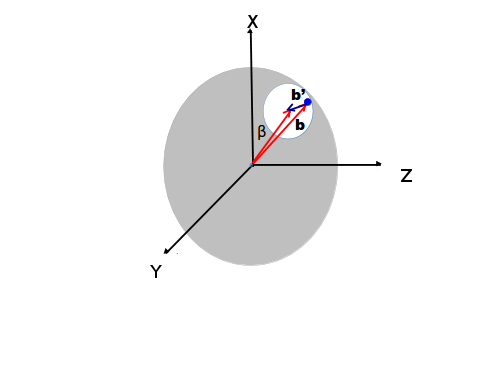
\includegraphics[scale=0.6]{fig/quarks_nucleus.png}
\vspace{-0.7in}
\caption{The spatial coordinates of quarks in a nucleus. See main text for definition of the variables. The figure is from \cite{simonetta_pre}. } 
\label{fig:quarks_nucleus}
\end{figure}

The $^4$He nucleus shows a clear EMC effect. This nucleus is characterized by its spin-zero, a high density and it is a well-known few-body system. These aspects make the $^4$He nucleus an ideal target to be considered for the understanding of the nuclear effects at the partonic level.  
  
  In principle, the $^4$He GPD $H_{A}(x,\xi,t)$ characterized by:
 \begin{itemize}
 \item The universality of $H_{A}$: the $H_{A}$ describes the partonic structure of the $^4$He in a DVCS reaction the same way as in a DVMP reaction. 
 \item In the forward limit ($t\rightarrow 0$), $H_{A}$ is reduced to the usual PDF of $^4$He that is accessible via DIS.
 \item $H_{A}$ can be decomposed into a polynomial in $\xi$.
 \item The first moment of $H_{A}$ is the $^4$He elastic electromagnetic form factor $F_{A}(t)$, such as:
 \begin{equation}
   \sum_{q} \int_{-1}^{1} dx ~H_{A}^{q}(x, \xi, t) =  F_{A}(t),
\end{equation}
  where the sum runs over all the quark flavors.
  \item The second moment of $H_{A}^{q}(x, \xi, t)$ reads
  \begin{equation}
  \int_{-1}^{1} dx ~x H_{A}^{q}(x, \xi, t) = M ^{q/A}_{2}(t) + \frac{4}{5} \xi^{2} d^{q/A}_{2}(t)
  \end{equation}
    where the first term of the right-hand side represents the momentum fraction carried by each quark flavor q, and the second term is encoding information about the forces experienced by partons inside the nuclei \cite{M_Polyakov}. 
  \item $H_{A}$ is not directly measured from experiment, but we measure its corresponding Compton form factor $\mathcal{H}_{A}$. 
\end{itemize}  

The $^4$He DVCS amplitude can be expressed as \cite{Kir}:
 \begin{equation}
 \mathcal{T}_{DVCS} \propto \sum_{q} e^{2}_{q} \mathcal{P} \int_{-1}^{1} dx \left(\frac{1}{x-\xi} + \frac{1}{x+\xi} \right) H^{q}_{A}(x,\xi,t) \\- i\pi \sum_{q} \left( e^{2}_{q} \left[ H^{q}_{A}(\xi,\xi,t) - H^{q}_{A}(-\xi,\xi,t) \right] \right),
\end{equation}
 where the first term on the right-hand side stands for the real part of the CFF $\mathcal{H}_{A}$, while the second term for the imaginary part of $\mathcal{H}_{A}$.     

The coherent DVCS amplitude is enhanced through the interference with the BH process, that is calculable from the well-known elastic FF. Figure \ref{fig:He-4_FFs} shows the world measurements of the $^4$He $F_{A}(t)$ along with theoretical calculations. Following the $F_{A}(t)$ parametrization by R. Frosch and his collaborators \cite{He_4_FF_Frosch} (valid at the small values of $-t$ which are of interest in this work), figure \ref{fig:BH_cross_section_4He} shows the calculated BH as a function of the azimuthal angle between the leptonic and the hadronic planes ($\phi$), using a 6~GeV electron beam on a $^4$He target.

  The experimentally measured $e ^4He \rightarrow e ^4He \gamma$ cross section can be decomposed into BH, DVCS, and interference terms. The differential cross section can be written like in Appendix \ref{app:Helium_cross_section}, equation \ref{eq:sigdiff}. By generalizing the BMK model \cite{Kir}, the nuclear BH, DVCS and interference scattering amplitudes can be decomposed into a finite series of Fourier harmonics as can be found in Appendix \ref{app:Helium_cross_section}, equations \ref{TTBH}, \ref{TTDVCS} and \ref{TTinter}.

\begin{figure}[tp]
\begin{minipage}[c]{.46\linewidth}
\hspace{-0.2in}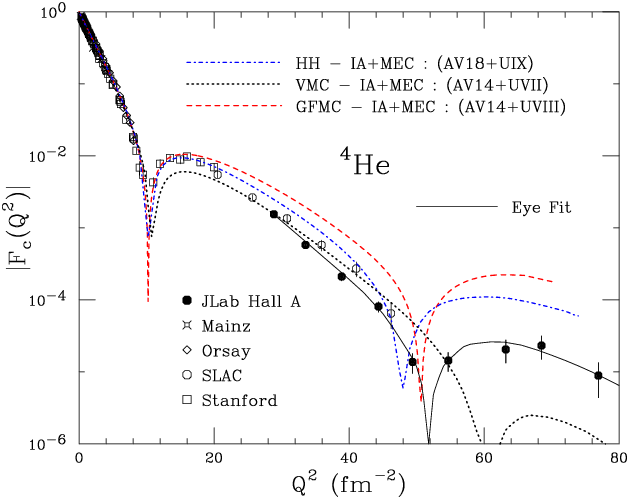
\includegraphics[height=6.1cm]{fig/He-4_FF.png}
\caption{$^4$He charge form factor measurements at Stanford, SLAC, Orsay, Mainz and JLab Hall A compared with theoretical calculations. The figure is from \cite{He_4_FF}. } 
\label{fig:He-4_FFs}
\end{minipage} \hfill
\begin{minipage}[c]{.46\linewidth}
\hspace{-0.3in}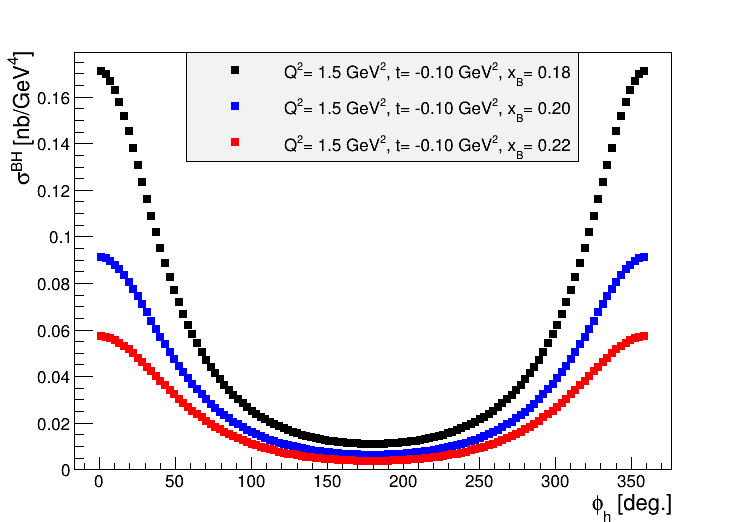
\includegraphics[height=6.3cm]{fig/BH_He-4.png}
\caption{The calculated BH cross section as a function of $\phi$ on a $^4He$ target at three values of $x_{B}$ and fixed values of $Q^{2}$ and $t$. ($t$~=~-~0.1~GeV$^2$/c$^2$ corresponds to $Q^2$~$\approx$~2.57~fm$^{-2}$ on figure \ref{fig:He-4_FFs}).}
\vspace{+0.3in}
\label{fig:BH_cross_section_4He}
\end{minipage}
\end{figure}


\subsection{Beam-spin asymmetry}
It is convenient to use the beam-spin asymmetry as DVCS observable because most of the experimental normalization and acceptance issues cancel out in an asymmetry ratio. The beam-spin asymmetry is measured using a polarized lepton beam on an unpolarized target (U). JLab provides a longitudinally (L) polarized electron beam, $P_{B}~\approx$~85~$\%$. It is defined as:
  \begin{equation}
  A_{LU} = \frac{d^{5}\sigma^{+} - d^{5}\sigma^{-} }
                {d^{5}\sigma^{+} + d^{5}\sigma^{-}}.
    \label{BSA_equation}
  \end{equation}
  where $d^{5}\sigma^{+}$($d^{5}\sigma^{-}$) is the DVCS differential cross section for a positive (negative) beam helicity.

 At leading twist, the beam-spin asymmetry ($A_{LU}$) with the  two opposite helicities of a  longitudinally-polarized electron beam (L) on a spin-zero target (U) can be written as:        
\begin{eqnarray}
A_{LU}& =& \frac{x_A(1+\epsilon^2)^2}{y} \, s_1^{INT} \sin(\phi) \, 
\bigg/ \, \bigg[ \, \sum_{n=0}^{n=2}c_n^{BH}\cos{(n\phi)} +  \\
& & \frac{x_A^2 t {(1+\epsilon^2)}^2}{Q^2} P_1(\phi) P_2(\phi) \, c_0^{DVCS} + 
\frac{x_A (1+\epsilon^2)^2}{y} \sum_{n=0}^{n=1} c_n^{INT} \cos{(n\phi)} \bigg].  \nonumber 
\label{eq:coh_BSA}
\end{eqnarray}

where $\mathcal{P}_1(\phi)$ and $\mathcal {P}_2(\phi)$ are the Bethe-Heitler 
propagators. The factors: $c_{0,1,2}^{BH}$, $c_0^{DVCS}$, $c_{0,1}^{INT}$ and 
$s_1^{INT}$ are the Fourier coefficients of the BH, the DVCS and the 
interference amplitudes for a spin-zero target \cite{Kir}. The explicit 
expressions of these coefficients can be found in Appendix 
\ref{app:Helium_cross_section}.


\subsection{Theoretical predictions} \label{Theoretical_hypotheses}

\paragraph{On-shell calculations} ~

The nuclear GPD $H_{A}$ can be described as the sum of the individual nucleons' GPDs. In the model based on the impulse approximation of V. Guzey {\it et al.} \cite{EMC_vadim_1, EMC_vadim_3}, a nucleus  is assumed to consist of non-relativistic non-interacting nucleons, and these nucleons interact independently with the probe. Assuming that the nucleon GPDs $H$ and $E$ are the dominant GPDs in the unpolarized target scattering case, the nuclear GPD $H_{A}$ for each quark flavor $q$ can be written as:
\begin{align}
H_{A}^{q}(x_A, \xi_{A}, t) &= \frac{dx_{N}}{dx_{A}} \Bigg[ Z \bigg( H^q_p(x_{N}, 
\xi_{N}, t) + \frac{t}{4 M^2} E^q_p(x_{N}, \xi_{N}, t) \bigg)\\ \nonumber
& + (A-Z) \bigg( H^q_n(x_{N}, \xi_{N}, t) + \frac{t}{4 M^2} E^q_n(x_{N}, \xi_{N}, t) 
\bigg) \Bigg] F_{A}(t),
\label{eq:guzey}
\end{align}
where the factor $dx_{N}/dx_{A}$ is the Jacobian for the transformation of $x$ 
from the nucleonic $x_N$ to the nuclear $x_{A}$. It is equal to $ 
A(2-x_{A})/(2-x_{B})$ with $x_A = x_B/A$. $\xi_{A}$ is defined as 
$x_{A}/(2-x_{A})$ and $\xi_{N}$ is equal to $x_B/(2-x_B)$. For free nucleons, the 
GPDs are constructed using the double distributions ansatz 
\cite{free_proton_GPDs}.  In this approximation, the GPD $H$ with its evolution 
in $Q^2$, can be written as:
\begin{equation}
H^{q}(x,\xi,t, Q^2) = \int_{0}^{1}d\beta \int_{-1+|\beta|}^{1+|\beta|} d\alpha \delta(\beta +\alpha \xi -x) \pi(\beta, \alpha) \beta^{-\alpha'(1-\beta)t} q_{\nu}(\beta, Q^2),
\end{equation} 
where the parameters $\alpha$ and $\beta$ are new variables that link $x$ and $\xi$ linearly as $x = \beta + \alpha \xi$, $q_{\nu}$ is the valence unpolarized PDF and the profile function $\pi(\beta, \alpha)$ takes the form
\begin{equation}
\pi(\beta, \alpha) = \frac{3}{4} \frac{(1-\beta)^2 - \alpha^2}{(1-\beta)^3}.
\end{equation}
The t-dependence of the GPD is introduced through Regge ansatz \cite{guidal_2}, with the slope $\alpha'$ equal to 1.105 GeV$^{-2}$ that allows to recover the ordinary form factors of the nucleons. 

This model enables to link the nuclear CFFs to the ones of the nucleons. However, it neglects the medium modifications and the binding effects between the nucleons in a nucleus. To take into account the nuclear modifications, the bound nucleons can be assumed to be modified in proportion to the corresponding bound nucleon elastic form factors \cite{EMC_vadim_2}. That is, the GPD $H$ of the bound proton ($H^{q/p*}$) can be written as:
\begin{equation}
H^{q/p*}(x,\xi,t, Q^2) = \frac{F^{p*}_{1}}{F^{p}_{1}} H^{q/p}(x,\xi,t, Q^2),
\end{equation}
where $F^{p}_{1}$ ($F^{p*}_{1}$) is the Dirac form factor of the free (bound) proton.
The bound nucleon form factor is calculated using the Quark-Meson Coupling (QMC) model \cite{QMC}, that predicts a suppression as the nuclear density increases. As a result of these calculations, figure~\ref{fig:EMC_vadim} shows the ratio of the bound (incoherent DVCS channel off $^4$He) to free proton beam-spin asymmetry ($A_{LU}$), at $\phi$ = 90$^{\circ}$, as a function of $x_B$, using a 6-GeV longitudinally-polarized electron beam at $Q^2$=~2~GeV$^2$/c$^2$ and two values of the transfer momentum $t$. This ratio represents a generalization of the EMC effect, for $t$ greater than zero. This model predicts an enhancement of the bound-proton beam-spin asymmetry, which increases with $t$.
\begin{figure}[tbp]
\centering
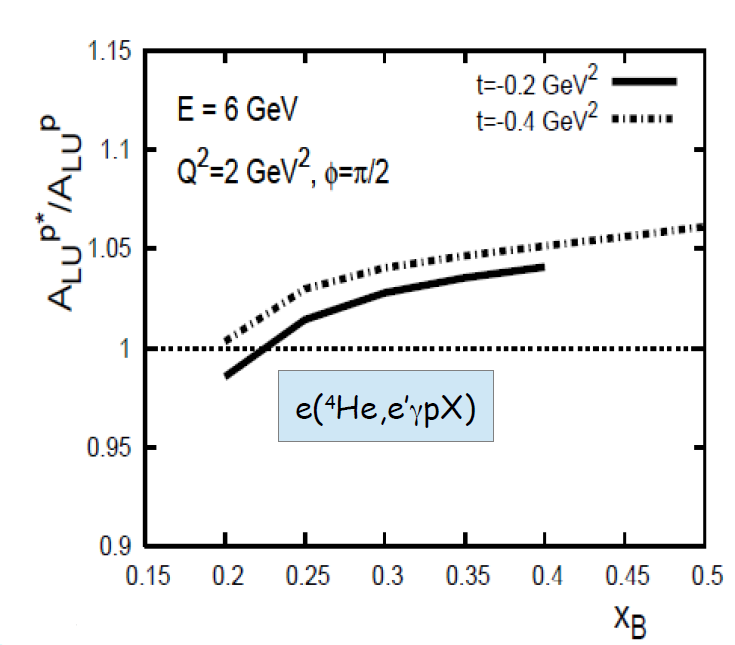
\includegraphics[scale=0.35]{fig/EMC_ALU_vadim.png}
\caption{The theoretical predictions by V.~Guzey \cite{EMC_vadim_2} for the 
"generalized" EMC effect in terms of the beam-spin asymmetry ratio between the 
bound proton in $^4$He and the free proton as a function of Bj\"orken variable 
$x_B$. The calculations are performed at two values of $-t$, 0.2 and 0.4 
GeV$^2$/c$^2$, with a 6 GeV electron beam and $Q^2$ = 2 GeV$^2$/c$^2$. } 
\label{fig:EMC_vadim}
\end{figure}

\paragraph{Off-shell calculations} ~

Another model for nuclear GPDs in the impulse approximation uses the nuclear spectral function. For a spin-zero nucleus, the GPD $H^{A}$ can be written as \cite{EMC_simonetta}:
\begin{align}
H^{A}(x, \zeta, t) &= \sum_{N} \int \frac{d^{2}P_{\perp} dY}{2(2\pi)^3} \, 
   \frac{1}{A-Y}\,  \, \rho^{A}(P^2, P'^2) \mathcal{A}\\ \nonumber
& ~~~~~~~~ \times \sqrt{\frac{Y-\zeta}{Y}} \left[H^{N}_{OFF}(\frac{x}{Y}, 
\frac{\zeta}{Y},P^2, t) - \frac{1}{4} \frac{(\zeta/Y)^2}{1-\zeta/Y } 
E^{N}_{OFF}(\frac{x}{Y}, \frac{\zeta}{Y},P^2, t) \right]
\label{eq:simonetta}
\end{align}
where $P$ and $P'$ are the incoming and outgoing nucleons three-momenta, $Y$ is 
a dynamical variable defined as $\frac{y+A\zeta}{1+\zeta}$, $\mathcal{A} = 
(Y-\zeta/2)(\sqrt{Y(Y-\zeta)})$ is a normalization factor with $\zeta = 
\frac{2\xi}{1+\xi/A}$, $\rho^{A}(P^2, P'^2)$ is the off-forward nuclear 
spectral function accounting for all configurations of the final nuclear system 
and the binding effects between the nucleons. In a non-relativistic 
approximation, $\rho^{A}$ is defined as \cite{simonetta_2}:
\begin{equation}
\rho^{A}(P^2, P'^2) = 2\pi M_A \int dP\,P\,\Phi(P)\,\Phi(P') 
\end{equation}
with $\Phi$ the nuclear wave function in momentum space. The off-forward nucleon GPDs, $H^{N}_{OFF}$ and $E^{N}_{OFF}$, are characterized by the off-shellness which is linked to $P^2$. One recovers the free nucleon GPDs by disregarding this off-shellness.  

The nuclear effects can be expressed with the ratio between the nuclear and the nucleon GPDs. This ratio becomes equal to the ordinary EMC ratio in the forward limit ($t = 0$). As the nuclear form factor of the $^4$He has a steeper drop in $t$ than the nucleonic one, it is more convenient to define the ratio between normalized GPDs as:
\begin{equation}
R_{A}(x, \xi,t) = \frac{H^{A}(x, \xi, t)/F^{A}(t)}{H^{p}(x, \xi, t)/F^{1}_{p}(t)}
\end{equation}
where $F^{1}_{p}(t)$ is the Dirac form factor of the proton. Figure \ref{fig:4HeEMC_RA} shows the EMC ratios measured via DIS on $^4$He compared to theoretical calculations. One can see that the latter calculations by S.~Liuti and K.~Taneja describe the EMC effect differently than the first scenario due to the off-shell effects of the nucleons associated in their calculation. 

The nuclear effects can be also viewed as the beam-spin asymmetry ratio ($\frac{A^{Incoh}_{LU}}{A^{p}_{LU}}$) between the incoherent proton and the free proton. Figure \ref{fig:EMC_Simonetta} shows the predicted EMC effect in $^4$He in terms of $\frac{A^{Incoh}_{LU}}{A^{p}_{LU}}$ as a function of $x_B$. The calculated ratio appears to be very sensitive on $t$, which encodes the information on the transverse degrees of freedom of the partons in the nucleon.

\begin{figure}[tbp]
\begin{minipage}[c]{.46\linewidth}
%\hspace{-0.4in}
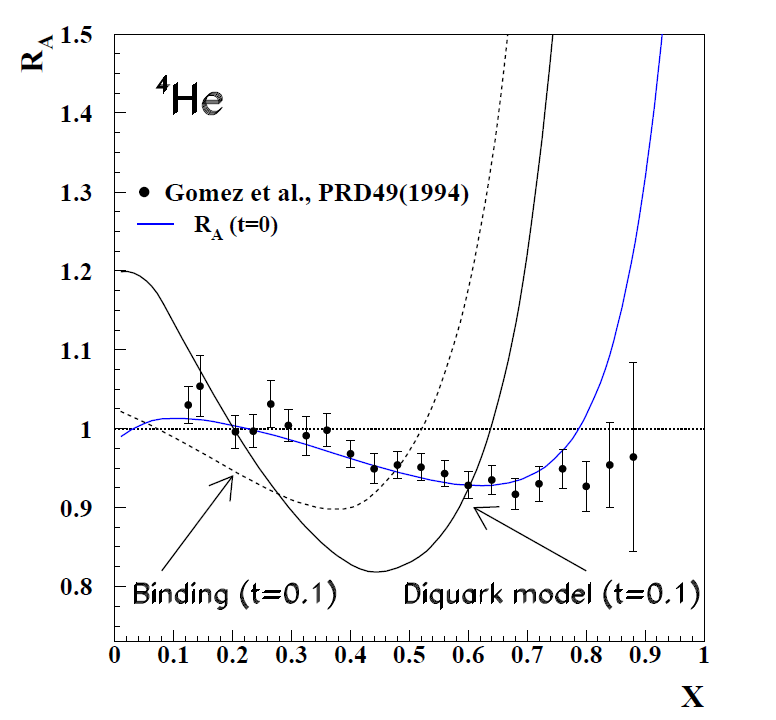
\includegraphics[height=7.8cm]{fig/4HeEMC_RA.png}
\caption{The EMC effect in $^4$He. The data points are the $^4$He EMC ratios \cite{He4_DIS_data}. The black dotted and solid curves are theoretical calculations based on a binding and a diquark model respectively, at $-t$= 0.1 GeV$^2$/c$^2$. The blue curve shows the theoretical calculation at the forward limit by Liuti and Taneja \cite{EMC_simonetta}.} 
\label{fig:4HeEMC_RA}
\end{minipage} \hfill
\begin{minipage}[c]{.46\linewidth}
\hspace{-0.3in}
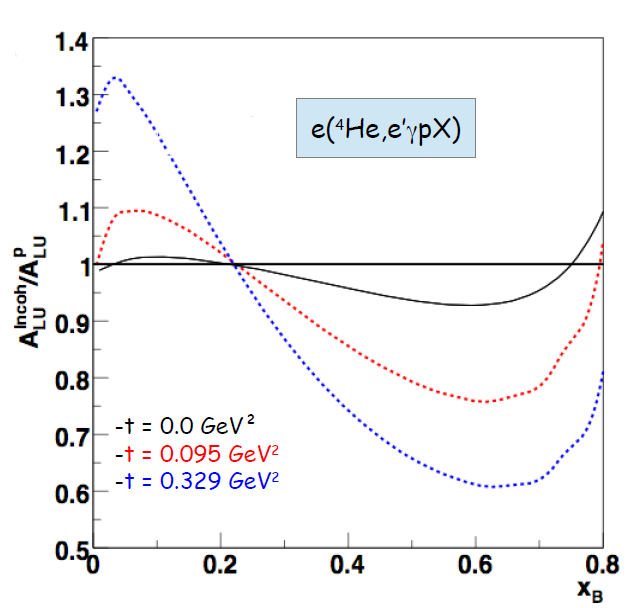
\includegraphics[height=7.8cm]{fig/EMC_ALU_simonetta.png}
\caption{The theoretical calculations by S. Liuti and K. Taneja \cite{EMC_simonetta} of the beam-spin asymmetry ratio between the bound proton, in $^4$He, and the free proton. The ratio is plotted as a function of $x$ at three different values of $-t$: 0, 0.095, and 0.329 GeV$^2$/c$^2$.}
\label{fig:EMC_Simonetta}
\vspace{+0.2in}
\end{minipage}
\end{figure}

We conclude that nuclear DVCS is a promising field that can give more details about the nature of the nuclear forces through the study of the nuclear GPDs, and through the study of the modifications of the nucleons' GPDs in nuclei.

\subsection{Nuclear DVCS measurements}
The first nuclear DVCS experiments were carried out by the HERMES 
collaboration \cite{HERMES_BSA}. In these measurements, 
longitudinally-polarized electron and positron beams at energies equal to 27.6 
GeV were scattered onto fixed nuclear targets (hydrogen, helium-4, nitrogen, 
neon, krypton and xenon) to study the DVCS reaction. The HERMES spectrometer 
did not detect the nuclear recoils. However, the exclusivity of the selected 
DVCS events was approximately ensured by a cut on the missing mass of the final 
state configuration $e\gamma X$. The separation between the coherent and the 
incoherent DVCS channels was made with a cut on $t$: the coherent channel is 
assumed to dominate the low $t$-region, while the higher $t$-region is assumed 
to be dominated by the incoherent channel on the protons and the neutrons.  
Figure \ref{fig:HERMES_BSA} shows the $\sin(\phi)$ amplitude of the beam-spin 
asymmetries off the different targets in $t$-bins measured by HERMES.  These 
asymmetries are further separated into coherent and incoherent asymmetries.  
Figure \ref{fig:HERMES_BSA_1} shows the mass dependence of the $\sin(\phi)$ 
amplitude of the coherent and the incoherent beam-spin asymmetries integrated 
over all the data sample for each target type.

\begin{figure}[tbp]
\centering
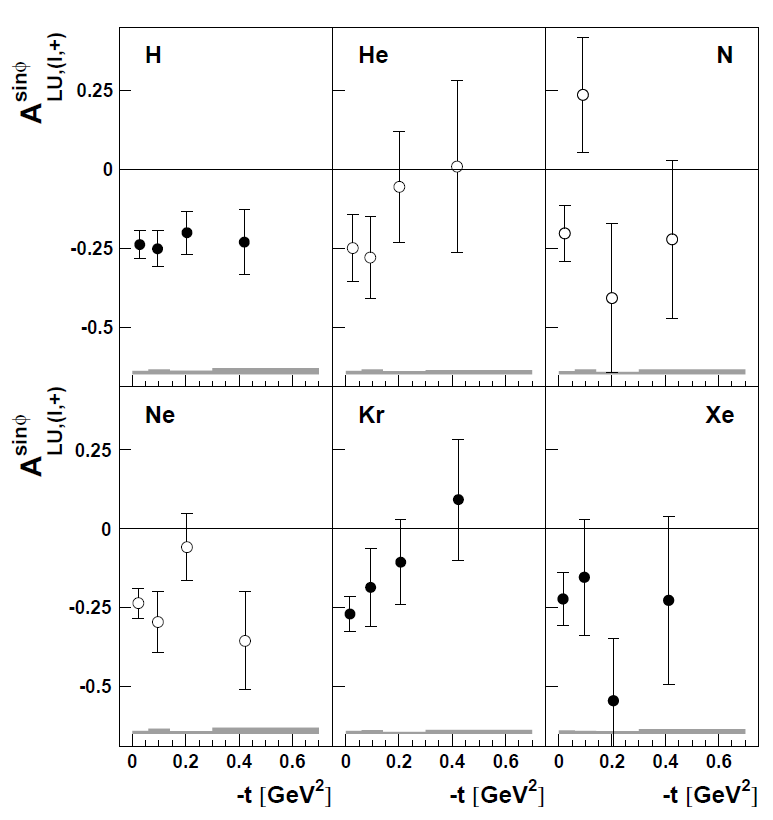
\includegraphics[height=9.7cm]{fig/HERMES_BSA.png}
\caption{The $t$-dependence of the $\sin(\phi)$ amplitude of the beam-spin asymmetries measured by HERMES on different nuclear targets. The error bars show only the statistical uncertainties, while the systematic uncertainties are indicated by the bands on each plot. \cite{HERMES_BSA}.} 
\label{fig:HERMES_BSA}
\end{figure}
\begin{figure}[tbp]
\centering
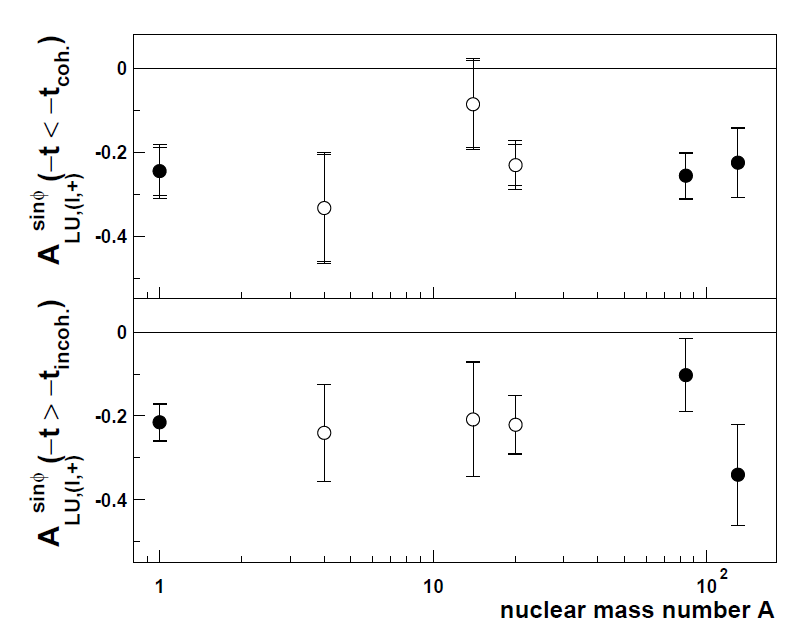
\includegraphics[height=8.0cm]{fig/HERMES_BSA_2.png}
\caption{The nuclear-mass dependence of the $\sin(\phi)$ amplitude of the beam-spin asymmetries for the coherent (upper panel) and the incoherent (lower panel) data samples. The values of $t_{coh}$ and $t_{incoh}$ for each nuclear target were determined from Monte-Carlo simulations \cite{HERMES_BSA}.}
\label{fig:HERMES_BSA_1}
\end{figure}

The HERMES inclusive measurements of the nuclear beam-spin asymmetries clearly suffer from a lack of statistics for a precise investigation of their physics content. Within the given uncertainties, their nuclear beam-spin asymmetries have shown neither enhancement, nor a nuclear-mass dependence.  




